\documentclass[aspectratio=169]{beamer}

% Theme and appearance
\usetheme{Madrid}
\usecolortheme{default}

% Packages
\usepackage[utf8]{inputenc}
\usepackage[T1]{fontenc}
\usepackage{graphicx}
\usepackage{tikz}
\usetikzlibrary{shapes,arrows,positioning,calc,backgrounds,fit,decorations.pathmorphing}
\usepackage{array}
\usepackage{booktabs}
\usepackage{multirow}
\usepackage{colortbl}
\usepackage{xcolor}

% Graphics path for icons
\graphicspath{{images/}}

% Custom colors
\definecolor{networkblue}{RGB}{51,102,187}
\definecolor{networkgreen}{RGB}{46,125,50}
\definecolor{networkorange}{RGB}{255,152,0}
\definecolor{networkred}{RGB}{198,40,40}

% Title information
\title{Introduction to Networking}
\author{Brendan Shea, PhD}
\institute{Rochester Community and Technical College}
\date{} % No date as requested

% Custom commands for network icons
\newcommand{\neticon}[2][0.4cm]{\includegraphics[height=#1]{#2}}

% TikZ styles for network diagrams
\tikzset{
    device/.style={rectangle, draw, thick, minimum width=2cm, minimum height=1cm, align=center},
    router/.style={rectangle, draw, thick, fill=networkblue!20, minimum width=2cm, minimum height=1cm, align=center},
    switch/.style={rectangle, draw, thick, fill=networkgreen!20, minimum width=2cm, minimum height=1cm, align=center},
    computer/.style={rectangle, draw, thick, fill=gray!20, minimum width=1.5cm, minimum height=1cm, align=center},
    connection/.style={thick, -latex},
    wireless/.style={thick, -latex, dashed, color=networkblue},
    cloud/.style={ellipse, draw, thick, fill=networkorange!10, minimum width=3cm, minimum height=2cm, align=center}
}

\begin{document}

% Title slide
\begin{frame}
\titlepage
\end{frame}

% Slide 1: Course Introduction
\begin{frame}{Welcome to Networking Basics}
\textbf{Learning Objectives:}
\begin{itemize}
    \item Understand fundamental networking concepts and terminology
    \item Learn about network types, topologies, and the OSI Model
    \item Develop systematic troubleshooting skills
    \item Build and configure SOHO networks
\end{itemize}

\begin{block}{Why This Matters}
Every time you stream a video, send a text, or browse the web, you're using computer networks!
\end{block}
\end{frame}

% Slide 2: What is Networking?
\begin{frame}{What is Networking?}
\begin{columns}
\begin{column}{0.65\textwidth}
\begin{itemize}
    \item A \textbf{computer network} is a system of interconnected devices that can communicate and share resources with each other.
    \item A \textbf{node} is any device connected to a network, while a \textbf{host} is a node that provides services or runs applications.
    \item Networks use \textbf{clients} (devices that request services) and \textbf{servers} (devices that provide services) to organize communication.
\end{itemize}

\vspace{0.3cm}
\begin{block}{Real-World Example}
When you watch Netflix, your phone (client) requests video data from Netflix's servers over the Internet!
\end{block}
\end{column}

\begin{column}{0.3\textwidth}
\centering
\neticon[1.6cm]{icon_laptop.png}\\
\vspace{0.2cm}
\neticon[1.3cm]{icon_router.png}\\
\vspace{0.2cm}
\neticon[1.6cm]{icon_server.png}
\end{column}
\end{columns}
\end{frame}

% Slide 3: Network Types - Overview
\begin{frame}{Network Types - Overview}

\begin{itemize}
    \item A \textbf{Personal Area Network (PAN)} connects devices within an individual's immediate workspace, typically within 10 meters.
    \item A \textbf{Local Area Network (LAN)} connects devices within a limited area such as a home, school, or office building.
    \item A \textbf{Metropolitan Area Network (MAN)} spans a city or large campus, connecting multiple LANs across several kilometers.
    \item A \textbf{Wide Area Network (WAN)} covers large geographical areas like countries or continents, connecting multiple MANs and LANs.
\end{itemize}

\end{frame}

% Slide 4: Network Types - Examples & Scale
\begin{frame}{Network Types - Examples \& Scale}

\begin{itemize}
    \item Network types are classified primarily by their geographical coverage and the number of devices they connect.
    \item Each network type uses different technologies and protocols optimized for its specific range and purpose.
    \item Understanding these categories helps network administrators choose the right tools and design strategies.
\end{itemize}

\vspace{0.3cm}

\begin{table}
\centering
\small
\begin{tabular}{|l|l|l|p{4cm}|}
\hline
\rowcolor{networkblue!30}
\textbf{Type} & \textbf{Range} & \textbf{Size} & \textbf{Typical Use Cases} \\ \hline
PAN & Up to 10m & 2-8 devices & Bluetooth headphones, smartwatch syncing \\ \hline
\rowcolor{gray!10}
LAN & Up to 1km & 10-1000 devices & Home networks, office buildings, school labs \\ \hline
MAN & Up to 100km & 1000+ devices & City-wide networks, university campuses \\ \hline
\rowcolor{gray!10}
WAN & Global & Millions & The Internet, corporate networks across countries \\ \hline
\end{tabular}
\end{table}

\end{frame}

% Slide 5: Introduction to Network Topologies
\begin{frame}{Introduction to Network Topologies}

\begin{itemize}
    \item \textbf{Network topology} refers to the physical or logical arrangement of devices and connections in a network.
    \item \textbf{Physical topology} describes how devices are actually connected with cables and hardware.
    \item \textbf{Logical topology} describes how data flows through the network, which may differ from the physical layout.
    \item Choosing the right topology affects network performance, reliability, cost, and ease of troubleshooting.
\end{itemize}

\vspace{0.3cm}

\begin{alertblock}{Why Topology Matters}
A well-designed topology can prevent network failures from affecting all users, while a poor design might bring down the entire network if one cable fails!
\end{alertblock}

\end{frame}

% Slide 6: Star Topology
\begin{frame}{Star Topology}

\begin{columns}
\begin{column}{0.5\textwidth}
\begin{itemize}
    \item In a \textbf{star topology}, all devices connect to a central hub or switch that manages network traffic.
    \item This design makes it easy to add new devices and identify problems since each device has its own connection.
    \item If one cable fails, only that device is affected, providing good \textbf{fault isolation}.
    \item The main disadvantage is that if the central device fails, the entire network goes down.
\end{itemize}
\end{column}

\begin{column}{0.45\textwidth}
\centering
\begin{tikzpicture}[scale=0.8]
    % Central switch
    \node[switch] (switch) at (0,0) {\neticon[0.6cm]{icon_switch.png}\\Switch};
    
    % Computers in star pattern
    \node[computer] (pc1) at (-2.5,2) {\neticon[0.5cm]{icon_pc.png}};
    \node[computer] (pc2) at (2.5,2) {\neticon[0.5cm]{icon_laptop.png}};
    \node[computer] (pc3) at (-2.5,-2) {\neticon[0.5cm]{icon_phone.png}};
    \node[computer] (pc4) at (2.5,-2) {\neticon[0.5cm]{icon_laptop.png}};
    
    % Connections
    \draw[connection] (switch) -- (pc1);
    \draw[connection] (switch) -- (pc2);
    \draw[connection] (switch) -- (pc3);
    \draw[connection] (switch) -- (pc4);
\end{tikzpicture}
\end{column}
\end{columns}

\end{frame}

% Slide 7: Mesh Topology
\begin{frame}{Mesh Topology}

\begin{columns}
\begin{column}{0.7\textwidth}
\begin{itemize}
    \item A \textbf{mesh topology} connects devices directly to multiple other devices, creating redundant paths for data.
    \item \textbf{Full mesh} means every device connects to every other device, while \textbf{partial mesh} has some direct connections.
    \item Mesh networks provide excellent fault tolerance since data can take alternate routes if one connection fails.
    \item The main disadvantages are high cost and complexity due to the large number of connections required.
    \item A \textbf{partial mesh}--often used in WANs--balances redundancy and cost. Here, only critical devices have multiple connections.
\end{itemize}
\end{column}

\begin{column}{0.3\textwidth}
\centering
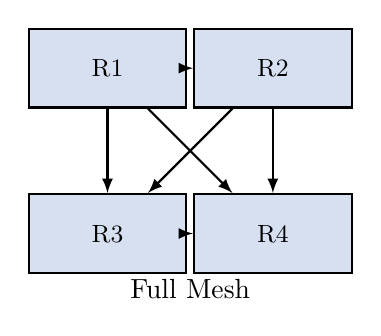
\begin{tikzpicture}[scale=0.7]
    % Four routers in mesh
    \node[router] (r1) at (0,2) {\small R1};
    \node[router] (r2) at (3,2) {\small R2};
    \node[router] (r3) at (0,-1) {\small R3};
    \node[router] (r4) at (3,-1) {\small R4};
    
    % Full mesh connections
    \draw[connection] (r1) -- (r2);
    \draw[connection] (r1) -- (r3);
    \draw[connection] (r1) -- (r4);
    \draw[connection] (r2) -- (r3);
    \draw[connection] (r2) -- (r4);
    \draw[connection] (r3) -- (r4);
    
    \node at (1.5,-2) {Full Mesh};
\end{tikzpicture}
\end{column}
\end{columns}

\end{frame}

% Slide 8: Legacy Topologies
\begin{frame}{Legacy Topologies}

\begin{itemize}
    \item A \textbf{bus topology} connects all devices to a single backbone cable, with data transmitted in both directions along the cable.
    \item A \textbf{ring topology} connects devices in a circular pattern where data travels in one direction around the ring.
    \item These topologies were common in early networks but have largely been replaced by star and mesh designs.
    \item Bus networks are difficult to troubleshoot, and ring networks can fail if any single connection breaks.
\end{itemize}

\vspace{0.3cm}

\begin{center}
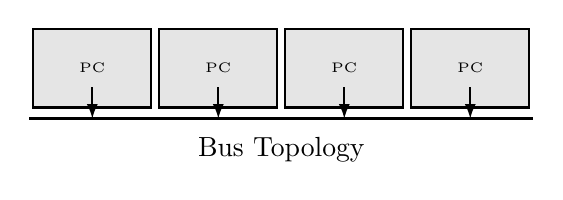
\begin{tikzpicture}[scale=0.8]
    % Bus topology
    \draw[very thick] (0,0) -- (8,0);
    \node[computer] at (1,0.8) {\tiny PC};
    \node[computer] at (3,0.8) {\tiny PC};
    \node[computer] at (5,0.8) {\tiny PC};
    \node[computer] at (7,0.8) {\tiny PC};
    \draw[connection] (1,0.5) -- (1,0);
    \draw[connection] (3,0.5) -- (3,0);
    \draw[connection] (5,0.5) -- (5,0);
    \draw[connection] (7,0.5) -- (7,0);
    \node at (4,-0.5) {Bus Topology};
\end{tikzpicture}
\end{center}

\end{frame}

% Slide 9: Topology Comparison
\begin{frame}{Topology Comparison}

\begin{itemize}
    \item Different topologies are suited for different scenarios based on cost, reliability needs, and scale.
    \item Modern networks often combine multiple topologies to balance efficiency and reliability.
    \item Star topology is most common in modern LANs due to its simplicity and manageability.
\end{itemize}

\vspace{0.2cm}

\begin{table}
\centering
\small
\begin{tabular}{|l|c|c|c|c|p{2.5cm}|}
\hline
\rowcolor{networkblue!30}
\textbf{Topology} & \textbf{Cost} & \textbf{Reliability} & \textbf{Scalability} & \textbf{Installation} & \textbf{Best Use} \\ \hline
Star & Medium & Medium & High & Easy & Modern LANs, offices \\ \hline
\rowcolor{gray!10}
Mesh & High & Very High & Low & Complex & Critical systems, WANs \\ \hline
Bus & Low & Low & Low & Easy & Legacy systems only \\ \hline
\rowcolor{gray!10}
Ring & Medium & Low & Medium & Medium & Legacy token ring \\ \hline
\end{tabular}
\end{table}

\end{frame}

% Slide 10: Choosing the Right Topology
\begin{frame}{Choosing the Right Topology}

\begin{itemize}
    \item Budget constraints often determine which topology is feasible, with bus being cheapest and mesh being most expensive.
    \item Reliability requirements guide topology choice, as critical systems need redundant connections that mesh provides.
    \item Scalability needs affect the decision, since star topologies make it easy to add devices while mesh becomes complex.
    \item Most real-world networks use \textbf{hybrid topologies} that combine different designs to balance cost and performance.
\end{itemize}

\vspace{0.3cm}

\begin{block}{Example: School Network}
A typical school might use star topology within each classroom (devices connect to a switch), with those switches connected in a partial mesh to provide redundancy between buildings.
\end{block}

\end{frame}

% Slide 11: Case Study Problem - Network Design Challenge
\begin{frame}{Case Study: Luna \& Neville Design a Network}

\begin{alertblock}{The Scenario}
Luna and Neville have been asked to design a network for Hogwarts to connect three castle towers: Gryffindor, Ravenclaw, and Hufflepuff.
\end{alertblock}

\vspace{0.3cm}

\textbf{Requirements:}
\begin{itemize}
    \item Each tower has 20 computers that need network access
    \item The network must remain functional even if one connection between towers fails (magical accidents happen!)
    \item Hogwarts has a limited budget and needs a cost-effective solution
    \item Installation should be manageable for the small IT team (just Luna and Neville)
\end{itemize}

\vspace{0.3cm}

\textbf{Your Challenge:}
\begin{enumerate}
    \item Which topology should Luna and Neville use \emph{within} each tower?
    \item Which topology should they use \emph{between} the three towers?
    \item Justify your choices based on the requirements above.
\end{enumerate}

\end{frame}

% Slide 12: Case Study Solution - Network Design Challenge
\begin{frame}{Case Study: Luna \& Neville's Solution}

\textbf{Their Recommended Solution:}
\begin{itemize}
    \item \textbf{Within each tower:} Use star topology with one switch per tower connecting all 20 computers.
    \item \textbf{Between towers:} Use partial mesh topology connecting the three tower switches with redundant paths.
    \item This hybrid approach balances cost, reliability, and ease of management effectively.
\end{itemize}

\vspace{0.2cm}

\textbf{Why This Works:}
\begin{itemize}
    \item Star within towers: Easy to install, easy to troubleshoot, cost-effective for 20 devices
    \item Partial mesh between towers: Provides redundancy (magical accidents won't take down the whole network!)
    \item If one inter-tower connection fails, traffic can be rerouted through the third tower
    \item Luna and Neville can manage this design without needing to hire additional wizards
\end{itemize}

\end{frame}

% Slide 13: Transition - From Hardware to Protocols
\begin{frame}{Transition: From Hardware to Protocols}

\begin{itemize}
    \item We've learned how to physically connect devices using different network topologies.
    \item But having wires and devices connected is only the beginning—we need rules for how data travels through these networks.
    \item These rules are called \textbf{protocols}, and they work together in organized layers to make networking possible.
    \item Think of it like a postal system: the physical topology is the roads and buildings, but we still need rules for addressing, packaging, and delivering mail.
\end{itemize}

\vspace{0.3cm}

\begin{alertblock}{Next Up: The OSI Model}
The OSI Model provides a framework for understanding how data moves from one application to another across a network, using seven distinct layers of protocols.
\end{alertblock}

\end{frame}

% Slide 14: What is the OSI Model?
\begin{frame}{What is the OSI Model?}

\begin{itemize}
    \item The \textbf{OSI Model (Open Systems Interconnection Model)} is a conceptual framework that standardizes how different network systems communicate.
    \item Created by the International Organization for Standardization (ISO) in 1984, it divides networking functions into seven distinct layers.
    \item Each layer has specific responsibilities and communicates only with the layers directly above and below it.
    \item The OSI Model helps network professionals understand, design, and troubleshoot networks systematically.
\end{itemize}

\vspace{0.3cm}

\begin{block}{The Postal System Analogy}
Think of the OSI Model like mailing a letter: you write it (Application), put it in an envelope with an address (Transport/Network), give it to the postal service (Data Link/Physical), who delivers it through their system.
\end{block}

\end{frame}

% Slide 15: The Seven Layers Overview
\begin{frame}{The Seven Layers Overview}

\begin{itemize}
    \item The OSI Model consists of seven layers numbered from 1 (bottom) to 7 (top), with data flowing down when sending and up when receiving.
    \item A popular memory trick is \textbf{"Please Do Not Throw Sausage Pizza Away"} representing Physical, Data Link, Network, Transport, Session, Presentation, Application.
    \item Upper layers (5-7) deal with software and applications, while lower layers (1-4) handle data transmission and routing.
\end{itemize}

\vspace{0.2cm}

\begin{table}
\centering
\small
\begin{tabular}{|c|l|l|}
\hline
\rowcolor{networkblue!30}
\textbf{Layer} & \textbf{Name} & \textbf{Basic Function} \\ \hline
7 & Application & User interface and applications \\ \hline
\rowcolor{gray!10}
6 & Presentation & Data formatting and encryption \\ \hline
5 & Session & Managing connections \\ \hline
\rowcolor{gray!10}
4 & Transport & Reliable delivery and flow control \\ \hline
3 & Network & Routing across networks \\ \hline
\rowcolor{gray!10}
2 & Data Link & Local network delivery \\ \hline
1 & Physical & Physical transmission of bits \\ \hline
\end{tabular}
\end{table}

\end{frame}

% Slide 16: Data Encapsulation & Decapsulation
\begin{frame}{Data Encapsulation \& Decapsulation}

\begin{itemize}
    \item \textbf{Encapsulation} is the process of adding headers (and sometimes trailers) to data as it moves down through the OSI layers when being sent.
    \item \textbf{Decapsulation} is the reverse process, where headers are removed as data moves up through the layers when being received.
    \item Each layer adds its own header containing information needed for that layer's function, creating a "package within a package" effect.
    \item The \textbf{Protocol Data Unit (PDU)} is the name for data at each specific layer, with different names at each level.
\end{itemize}

\vspace{0.3cm}

\begin{center}
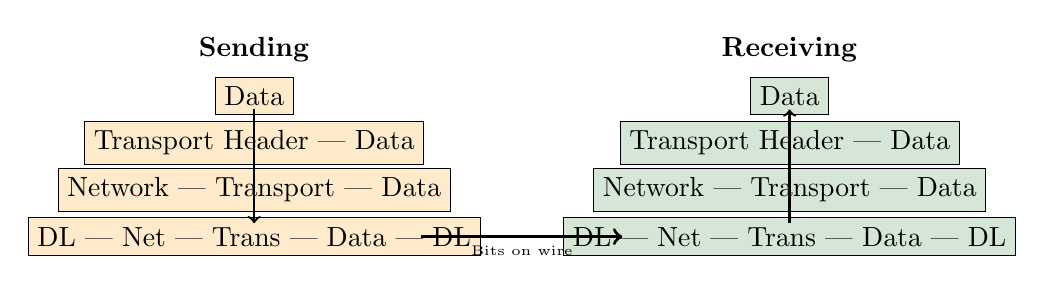
\begin{tikzpicture}[scale=0.85]
    % Sending side
    \node at (-1,3) {\textbf{Sending}};
    \node[draw, fill=networkorange!20] at (-1,2.3) {Data};
    \node[draw, fill=networkorange!20] at (-1,1.6) {Transport Header | Data};
    \node[draw, fill=networkorange!20] at (-1,0.9) {Network | Transport | Data};
    \node[draw, fill=networkorange!20] at (-1,0.2) {DL | Net | Trans | Data | DL};
    \draw[->, thick] (-1,2.1) -- (-1,0.4);
    
    % Receiving side
    \node at (7,3) {\textbf{Receiving}};
    \node[draw, fill=networkgreen!20] at (7,2.3) {Data};
    \node[draw, fill=networkgreen!20] at (7,1.6) {Transport Header | Data};
    \node[draw, fill=networkgreen!20] at (7,0.9) {Network | Transport | Data};
    \node[draw, fill=networkgreen!20] at (7,0.2) {DL | Net | Trans | Data | DL};
    \draw[->, thick] (7,0.4) -- (7,2.1);
    
    % Middle transmission
    \draw[->, very thick] (1.5,0.2) -- (4.5,0.2);
    \node[below] at (3,0.2) {\tiny Bits on wire};
\end{tikzpicture}
\end{center}

\end{frame}

% Slide 17: Layer 1 - Physical Layer
\begin{frame}{Layer 1: Physical Layer}

\begin{itemize}
    \item The \textbf{Physical Layer} handles the actual transmission of raw bits (1s and 0s) over a physical medium like cables or radio waves.
    \item This layer defines the physical characteristics of the network: voltages, cable types, connector shapes, and wireless frequencies.
    \item Physical layer devices include cables (Ethernet, fiber optic), hubs, repeaters, and the actual network interface cards (NICs).
    \item The PDU at this layer is simply called \textbf{bits}—the most basic unit of digital information.
    \item Problems at this layer include broken cables, incorrect connectors, or interference disrupting the signal.
\end{itemize}

\vspace{0.3cm}

\begin{alertblock}{Real-World Examples}
Cat5e/Cat6 Ethernet cables, fiber optic cables, Wi-Fi radio signals (2.4 GHz and 5 GHz), and the RJ-45 connector you plug into your laptop all operate at Layer 1.
\end{alertblock}

\end{frame}

% Slide 18: Layer 2 - Data Link Layer
\begin{frame}{Layer 2: Data Link Layer}

\begin{itemize}
    \item The \textbf{Data Link Layer} handles communication between devices on the same local network using physical addresses.
    \item Each network device has a unique \textbf{MAC address (Media Access Control address)} that identifies it at this layer—think of it like a serial number.
    \item This layer organizes bits from Layer 1 into \textbf{frames} and provides error detection to ensure data arrives correctly.
    \item Layer 2 devices include switches and wireless access points, which use MAC addresses to forward frames to the correct destination.
    \item The PDU at this layer is called a \textbf{frame}, which includes MAC addresses for both source and destination.
\end{itemize}

\vspace{0.3cm}

\begin{block}{Example MAC Address}
A MAC address looks like this: \texttt{00:1A:2B:3C:4D:5E} (six pairs of hexadecimal digits). Every network card manufactured has a unique MAC address assigned by the manufacturer.
\end{block}

\end{frame}

% Slide 19: Layer 3 - Network Layer
\begin{frame}{Layer 3: Network Layer}

\begin{itemize}
    \item The \textbf{Network Layer} enables communication between devices on different networks by providing logical addressing and routing.
    \item \textbf{IP addresses (Internet Protocol addresses)} identify devices at this layer and can be changed based on network location, unlike permanent MAC addresses.
    \item \textbf{Routers} operate at Layer 3, making decisions about the best path for data to travel across multiple networks.
    \item The PDU at this layer is called a \textbf{packet}, which contains both source and destination IP addresses.
    \item This layer handles breaking large messages into smaller packets and reassembling them at the destination.
\end{itemize}

\vspace{0.3cm}

\begin{alertblock}{Layer 2 vs Layer 3 Addressing}
MAC addresses (Layer 2) get you to the correct device on your local network, while IP addresses (Layer 3) get you to the correct network anywhere in the world!
\end{alertblock}

\end{frame}

% Slide 20: Layer 4 - Transport Layer
\begin{frame}{Layer 4: Transport Layer}

\begin{itemize}
    \item The \textbf{Transport Layer} ensures reliable end-to-end communication and manages data flow between applications on different devices.
    \item \textbf{TCP (Transmission Control Protocol)} provides reliable, connection-oriented communication with error checking and guaranteed delivery.
    \item \textbf{UDP (User Datagram Protocol)} offers faster, connectionless communication without delivery guarantees—useful for streaming and gaming.
    \item \textbf{Port numbers} identify specific applications on a device (like port 80 for web traffic or port 443 for secure web traffic).
    \item The PDU at this layer is called a \textbf{segment} (for TCP) or \textbf{datagram} (for UDP).
\end{itemize}

\vspace{0.3cm}

\begin{block}{TCP vs UDP Analogy}
TCP is like certified mail (you get confirmation of delivery), while UDP is like shouting across a room (faster but no guarantee they heard you).
\end{block}

\end{frame}

% Slide 21: Layers 5-7 - Upper Layers
\begin{frame}{Layers 5-7: Upper Layers}

\begin{itemize}
    \item \textbf{Layer 5 (Session Layer)} manages the opening, maintenance, and closing of communication sessions between applications.
    \item \textbf{Layer 6 (Presentation Layer)} handles data formatting, encryption, compression, and translation so different systems can understand each other.
    \item \textbf{Layer 7 (Application Layer)} provides network services directly to user applications like web browsers, email clients, and file transfer programs.
    \item These three layers are often grouped together because they all deal with software and user-facing functions rather than data transmission.
\end{itemize}

\vspace{0.2cm}

\begin{table}
\centering
\small
\begin{tabular}{|c|l|l|}
\hline
\rowcolor{networkblue!30}
\textbf{Layer} & \textbf{Name} & \textbf{Common Protocols/Examples} \\ \hline
7 & Application & HTTP, FTP, SMTP, DNS \\ \hline
\rowcolor{gray!10}
6 & Presentation & SSL/TLS, JPEG, MP3 \\ \hline
5 & Session & NetBIOS, RPC \\ \hline
\end{tabular}
\end{table}

\end{frame}

% Slide 22: OSI Model Summary
\begin{frame}{OSI Model Summary}

\begin{itemize}
    \item The OSI Model provides a systematic way to understand how data moves from one application to another across a network.
    \item When troubleshooting, it's best to work from the bottom (Physical) to the top (Application) to systematically identify problems.
    \item All seven layers work together seamlessly—if any layer fails, communication cannot occur.
\end{itemize}

\vspace{0.2cm}

\begin{table}
\centering
\small
\begin{tabular}{|c|l|l|l|l|}
\hline
\rowcolor{networkblue!30}
\textbf{Layer} & \textbf{Name} & \textbf{Function} & \textbf{PDU} & \textbf{Key Devices/Protocols} \\ \hline
7 & Application & User applications & Data & HTTP, FTP, DNS \\ \hline
\rowcolor{gray!10}
6 & Presentation & Format, encrypt data & Data & SSL/TLS, JPEG \\ \hline
5 & Session & Manage connections & Data & NetBIOS, RPC \\ \hline
\rowcolor{gray!10}
4 & Transport & End-to-end delivery & Segment/Datagram & TCP, UDP \\ \hline
3 & Network & Routing & Packet & IP, Routers \\ \hline
\rowcolor{gray!10}
2 & Data Link & Local delivery & Frame & MAC, Switches \\ \hline
1 & Physical & Transmit bits & Bits & Cables, Hubs \\ \hline
\end{tabular}
\end{table}

\end{frame}

% Slide 23: Case Study Problem - Troubleshooting with OSI
\begin{frame}{Case Study: Hermione Troubleshoots the Network}

\begin{alertblock}{The Problem}
Hermione is in the Hogwarts library trying to access a website on her laptop, but it won't load. However, her phone works fine accessing the same website while connected to the same Wi-Fi network.
\end{alertblock}

\vspace{0.3cm}

\textbf{What We Know:}
\begin{itemize}
    \item The laptop shows it is connected to the Wi-Fi network
    \item Other students' devices are working fine on the same network
    \item Hermione's phone can access the website without any problems
    \item Only this one specific website fails on the laptop—other websites work fine
\end{itemize}

\vspace{0.3cm}

\textbf{Your Challenge:}
\begin{enumerate}
    \item Using the OSI model, identify which layers you should check and in what order.
    \item What might be wrong at each layer you investigate?
    \item What is the most likely cause of this specific problem?
\end{enumerate}

\end{frame}

% Slide 24: Case Study Solution - Troubleshooting with OSI
\begin{frame}{Case Study: Hermione's Solution}

\textbf{Layer-by-Layer Analysis:}
\begin{itemize}
    \item \textbf{Layers 1-2 (Physical/Data Link):} These are working—laptop is connected to Wi-Fi successfully.
    \item \textbf{Layer 3 (Network):} Partially working—other websites load, so routing and IP addressing are functional.
    \item \textbf{Layer 4 (Transport):} Could be a port issue, but unlikely since other sites work.
    \item \textbf{Layers 5-7 (Upper layers):} Most likely culprit—could be browser cache, DNS issues, or firewall blocking this specific site.
\end{itemize}

\vspace{0.3cm}

\textbf{Most Likely Causes:}
\begin{enumerate}
    \item \textbf{Browser cache/cookies problem:} Old cached data causing conflicts (clear browser cache)
    \item \textbf{DNS cache issue:} Laptop has incorrect IP address cached for this website (flush DNS cache)
    \item \textbf{Browser-specific problem:} Try a different browser on the laptop
\end{enumerate}

\end{frame}

% Slide 25: Transition - The OSI Model in Action
\begin{frame}{Transition: The OSI Model in Action}

\begin{itemize}
    \item We've learned the theoretical framework of how networks communicate through the OSI Model's seven layers.
    \item Now we'll see how these layers work together in a practical, real-world setting that you use every day.
    \item \textbf{SOHO networks (Small Office/Home Office)} are networks that combine all OSI layers into compact, affordable devices.
    \item Understanding SOHO networks will show you how routers, switches, and wireless access points implement multiple OSI layers in a single device.
\end{itemize}

\vspace{0.3cm}

\begin{block}{What's Next}
Your home Wi-Fi router isn't just a router—it's actually a combination device that operates at multiple OSI layers simultaneously! We'll explore how these all-in-one devices work.
\end{block}

\end{frame}

% Slide 26: What is a SOHO Network?
\begin{frame}{What is a SOHO Network?}

\begin{itemize}
    \item A \textbf{SOHO network (Small Office/Home Office)} is a small-scale network typically designed to support 1-10 devices in a home or small business environment.
    \item SOHO networks are characterized by their simplicity, affordability, and all-in-one devices that combine multiple networking functions.
    \item The key components of a SOHO network include a router, modem, wireless access point, and the connected devices like computers and phones.
    \item Most home networks are SOHO networks—if you have Wi-Fi at home, you're already managing a SOHO network!
\end{itemize}

\vspace{0.3cm}

\begin{block}{Typical SOHO Network}
A family home might have a cable modem connected to a wireless router, which then provides wired and wireless connections to laptops, smartphones, smart TVs, and gaming consoles.
\end{block}

\end{frame}

% Slide 27: The SOHO Router
\begin{frame}{The SOHO Router}

\begin{columns}
\begin{column}{0.55\textwidth}
\begin{itemize}
    \item A \textbf{SOHO router} is actually multiple devices combined into one: a router, switch, wireless access point, and firewall all in a single box.
    \item The \textbf{WAN port} (Wide Area Network port) connects to your Internet Service Provider through a modem or directly to the ISP.
    \item The \textbf{LAN ports} (Local Area Network ports) provide wired Ethernet connections to devices in your home or office.
    \item This multi-function design saves money and space while operating at multiple OSI layers simultaneously.
\end{itemize}
\end{column}

\begin{column}{0.4\textwidth}
\centering
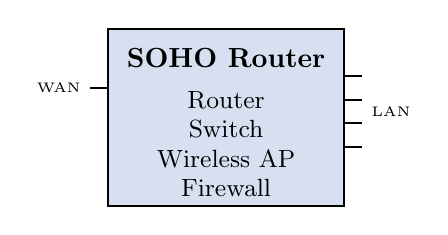
\begin{tikzpicture}[scale=0.75]
    % Router box
    \draw[thick, fill=networkblue!20] (0,0) rectangle (4,3);
    \node at (2,2.5) {\textbf{SOHO Router}};
    
    % Functions inside
    \node[align=left] at (2,1.8) {\small Router};
    \node[align=left] at (2,1.3) {\small Switch};
    \node[align=left] at (2,0.8) {\small Wireless AP};
    \node[align=left] at (2,0.3) {\small Firewall};
    
    % WAN port (left)
    \draw[thick] (-0.3,2) -- (0,2);
    \node[left] at (-0.3,2) {\tiny WAN};
    
    % LAN ports (right)
    \draw[thick] (4,2.2) -- (4.3,2.2);
    \draw[thick] (4,1.8) -- (4.3,1.8);
    \draw[thick] (4,1.4) -- (4.3,1.4);
    \draw[thick] (4,1.0) -- (4.3,1.0);
    \node[right] at (4.3,1.6) {\tiny LAN};
\end{tikzpicture}
\end{column}
\end{columns}

\end{frame}

% Slide 28: Physical Layer Functions in SOHO
\begin{frame}{Physical Layer Functions in SOHO}

\begin{itemize}
    \item SOHO routers provide \textbf{Ethernet ports} with RJ-45 connectors for wired connections, typically supporting speeds of 100 Mbps to 1 Gbps.
    \item The wireless radio transmits and receives data using \textbf{Wi-Fi signals} on two frequency bands: 2.4 GHz (longer range) and 5 GHz (faster speed).
    \item \textbf{LED indicators} on the router show the status of power, Internet connection, wireless activity, and LAN port connections.
    \item The modem connection (cable, DSL, or fiber) provides the physical link to your Internet Service Provider.
\end{itemize}

\vspace{0.3cm}

\begin{alertblock}{Common Physical Layer Issues}
No Internet connectivity? Check these Layer 1 items first: Is the router powered on? Are cables securely connected? Are the link lights on? Is the modem working?
\end{alertblock}

\end{frame}

% Slide 29: Data Link Layer Functions in SOHO
\begin{frame}{Data Link Layer Functions in SOHO}

\begin{itemize}
    \item The built-in \textbf{switch} connects multiple wired devices on the LAN using MAC addresses to forward frames efficiently to the correct port.
    \item The \textbf{wireless access point} broadcasts Wi-Fi signals following the 802.11 standards (like 802.11ac or 802.11ax/Wi-Fi 6) for wireless device connectivity.
    \item \textbf{DHCP (Dynamic Host Configuration Protocol)} automatically assigns IP addresses to devices when they connect to the network, eliminating manual configuration.
    \item \textbf{MAC address filtering} can restrict which devices are allowed to connect based on their hardware addresses, providing basic security.
\end{itemize}

\vspace{0.3cm}

\begin{block}{DHCP in Action}
When your phone connects to home Wi-Fi, DHCP automatically gives it an IP address (like 192.168.1.105), the router's address (gateway), and DNS server information—all without you doing anything!
\end{block}

\end{frame}

% Slide 30: Network Layer Functions in SOHO
\begin{frame}{Network Layer Functions in SOHO}

\begin{itemize}
    \item The router function operates at Layer 3, making routing decisions between your local network and the Internet.
    \item \textbf{NAT (Network Address Translation)} allows multiple devices on your home network to share a single public IP address when accessing the Internet.
    \item \textbf{Private IP addresses} (like 192.168.x.x or 10.x.x.x) are used within your home, while one \textbf{public IP address} is used for Internet communication.
    \item The router acts as the \textbf{default gateway}, forwarding packets from your local network to the Internet and vice versa.
\end{itemize}

\vspace{0.3cm}

\begin{block}{NAT in Action}
Your laptop has private IP 192.168.1.50 inside your home. When you visit a website, NAT translates this to your public IP (like 98.123.45.67) so the website knows where to send responses back!
\end{block}

\end{frame}

% Slide 31: Transport & Application Layer Functions
\begin{frame}{Transport \& Application Layer Functions}

\begin{itemize}
    \item \textbf{Port forwarding} allows specific external traffic to reach devices on your internal network by redirecting traffic from specific ports to designated local IP addresses.
    \item \textbf{Quality of Service (QoS)} prioritizes certain types of traffic (like video calls or gaming) to ensure they get adequate bandwidth even when the network is busy.
    \item \textbf{DNS forwarding} receives DNS requests from your devices and forwards them to your ISP's DNS servers to translate domain names into IP addresses.
    \item Application-level filtering can block or allow specific websites, services, or applications based on parental controls or business policies.
\end{itemize}

\vspace{0.3cm}

\begin{alertblock}{Why Port Forwarding Matters}
Want to host a gaming server or access security cameras remotely? You'll need port forwarding to allow external connections through your router to the specific device!
\end{alertblock}

\end{frame}

% Slide 32: Security in SOHO Networks
\begin{frame}{Security in SOHO Networks}

\begin{itemize}
    \item SOHO routers include a built-in \textbf{firewall} that filters incoming and outgoing traffic to protect your network from unauthorized access and attacks.
    \item \textbf{Wi-Fi encryption} protocols like WPA2 and WPA3 scramble wireless data so eavesdroppers cannot intercept and read your network traffic.
    \item Strong \textbf{password protection} on both your Wi-Fi network and router admin interface prevents unauthorized users from accessing your network or changing settings.
    \item \textbf{Guest networks} create separate wireless networks for visitors that cannot access your main network devices, protecting your privacy and security.
\end{itemize}

\vspace{0.3cm}

\begin{alertblock}{Security Best Practices}
Always change default admin passwords, use WPA3 (or WPA2 minimum), enable the firewall, and regularly update router firmware to patch security vulnerabilities!
\end{alertblock}

\end{frame}

% Slide 33: Connecting to the Internet
\begin{frame}{Connecting to the Internet}

\begin{itemize}
    \item Your \textbf{ISP (Internet Service Provider)} provides the connection between your home network and the broader Internet.
    \item A \textbf{modem} converts signals between your ISP's network and your home network (often cable, DSL, or fiber connections).
    \item Some ISPs provide combination modem-router devices, while others require separate modem and router equipment.
    \item Your ISP assigns you a public IP address that identifies your home network on the Internet.
\end{itemize}
\vspace{0.3cm}


\begin{center}
\begin{tikzpicture}[scale=1]
    % Home devices
    \node (laptop) at (0,1) {\neticon[1cm]{icon_laptop.png}};
    \node (phone) at (1.5,0) {\neticon[1cm]{icon_phone.png}};
    \node (pc) at (3,-1) {\neticon[1cm]{icon_pc.png}};
    
    % Router
    \node (router) at (5,0) {\neticon[1.2cm]{icon_router.png}};
    
    % Modem (using server icon as placeholder for modem)
    \node (modem) at (7.5,0) {\neticon[1.2cm]{icon_server.png}};
    
    % Internet cloud
    \node (internet) at (10,0) {\neticon[1.5cm]{icon_cloud.png}};
    
    % Connections with arrows
    \draw[->, very thick] (laptop) -- (router);
    \draw[->, very thick, dashed] (phone) -- (router);
    \draw[->, very thick] (pc) -- (router);
    \draw[->, very thick] (router) -- (modem);
    \draw[->, very thick] (modem) -- (internet);
    
    % Labels
    \node[below, font=\small] at (1.5,-0.8) {Home Devices};
    \node[below, font=\small] at (5,-0.8) {SOHO Router};
    \node[below, font=\small] at (7.5,-0.8) {Modem};
    \node[below, font=\small] at (10,-0.8) {Internet};
\end{tikzpicture}
\end{center}

\end{frame}

% Slide 34: Binary and Hexadecimal Basics
\begin{frame}{Binary and Hexadecimal Basics}

\begin{itemize}
    \item Computers use \textbf{binary (base-2)} number system because electronic circuits can easily represent two states: on (1) or off (0).
    \item \textbf{Hexadecimal (base-16)} uses digits 0-9 and letters A-F to represent values, providing a more compact way to write binary numbers.
    \item Each hexadecimal digit represents exactly four binary digits (bits), making conversion between the two systems straightforward.
    \item Network professionals use binary and hexadecimal to work with IP addresses, MAC addresses, and subnet masks.
\end{itemize}

\vspace{0.3cm}

\begin{block}{Why This Matters in Networking}
IP addresses like 192.168.1.1 are actually binary numbers! MAC addresses like 00:1A:2B:3C:4D:5E use hexadecimal. Understanding these number systems helps you work with network addresses effectively.
\end{block}

\end{frame}

% Slide 35: Number System Conversion
\begin{frame}{Number System Conversion}

\begin{itemize}
    \item Converting between decimal, binary, and hexadecimal is essential for understanding how network addresses are structured and manipulated.
    \item Binary numbers grow long quickly (192 in decimal is 11000000 in binary), which is why hexadecimal is preferred for human readability.
    \item One byte (8 bits) can represent decimal values from 0 to 255, which is why IP address octets use this range.
\end{itemize}

\vspace{0.2cm}

\begin{table}
\centering
\small
\begin{tabular}{|c|c|c||c|c|c|}
\hline
\rowcolor{networkblue!30}
\textbf{Decimal} & \textbf{Binary} & \textbf{Hex} & \textbf{Decimal} & \textbf{Binary} & \textbf{Hex} \\ \hline
0 & 0000 & 0 & 8 & 1000 & 8 \\ \hline
\rowcolor{gray!10}
1 & 0001 & 1 & 9 & 1001 & 9 \\ \hline
2 & 0010 & 2 & 10 & 1010 & A \\ \hline
\rowcolor{gray!10}
3 & 0011 & 3 & 11 & 1011 & B \\ \hline
4 & 0100 & 4 & 12 & 1100 & C \\ \hline
\rowcolor{gray!10}
5 & 0101 & 5 & 13 & 1101 & D \\ \hline
6 & 0110 & 6 & 14 & 1110 & E \\ \hline
\rowcolor{gray!10}
7 & 0111 & 7 & 15 & 1111 & F \\ \hline
\end{tabular}
\end{table}

\end{frame}

% Slide 36: Case Study Problem - Setting Up a Home Network
\begin{frame}{Case Study: Ron Sets Up the Burrow Network}

\begin{alertblock}{The Scenario}
Ron needs to set up a home network at the Burrow for his family. They have 2 laptops, 3 smartphones, 1 smart TV, and 1 gaming console that all need Internet access.
\end{alertblock}

\vspace{0.3cm}

\textbf{Requirements:}
\begin{itemize}
    \item Secure Wi-Fi for the family's mobile devices
    \item Wired connection for the gaming console (for better performance)
    \item A separate guest network for visitors so they can't access family devices
    \item Good Wi-Fi coverage throughout the three-story house
\end{itemize}

\vspace{0.3cm}

\textbf{Your Challenge:}
\begin{enumerate}
    \item What network topology should Ron use?
    \item Where should he place the wireless router for best coverage?
    \item What security settings should Ron configure?
\end{enumerate}

\end{frame}

% Slide 37: Case Study Solution - Setting Up a Home Network
\begin{frame}{Case Study: Ron's Solution}

\textbf{Recommended Solution:}
\begin{itemize}
    \item \textbf{Topology:} Star topology with all devices connecting to a central SOHO router/wireless access point.
    \item \textbf{Router placement:} Central location on the second floor for optimal Wi-Fi coverage across all three floors.
    \item \textbf{Wired connection:} Run an Ethernet cable from router to gaming console for low-latency gaming.
\end{itemize}

\vspace{0.2cm}

\textbf{Security Configuration:}
\begin{itemize}
    \item Enable WPA3 encryption (or WPA2 if WPA3 unavailable) with a strong, unique password
    \item Change default router admin password to prevent unauthorized access
    \item Enable guest network feature with a separate password for visitors
    \item Enable the built-in firewall and keep router firmware updated
\end{itemize}

\vspace{0.2cm}

\textbf{OSI Layers in Action:} This setup uses Physical (cables/Wi-Fi), Data Link (switch/AP), Network (routing/NAT), and Application (security settings) layers!

\end{frame}

% Slide 38: Transition - When Things Go Wrong
\begin{frame}{Transition: When Things Go Wrong}

\begin{itemize}
    \item Networks are complex systems with many components working together—problems are inevitable and happen regularly.
    \item Random troubleshooting by guessing wastes time, can make problems worse, and often fails to find the root cause.
    \item A \textbf{systematic troubleshooting methodology} provides a structured approach to identify and resolve network issues efficiently.
    \item Professional network technicians follow a standard seven-step process that applies to nearly every networking problem.
    \item Learning this methodology now will save you hours of frustration and make you a more effective troubleshooter.
\end{itemize}

\vspace{0.3cm}

\begin{alertblock}{The Cost of Poor Troubleshooting}
In business environments, network downtime can cost thousands of dollars per hour. Systematic troubleshooting gets networks back online faster and more reliably!
\end{alertblock}

\end{frame}

% Slide 39: Network Troubleshooting Methodology
\begin{frame}{Network Troubleshooting Methodology}

\begin{itemize}
    \item The industry-standard troubleshooting methodology consists of seven clear steps that guide you from problem identification to resolution.
    \item Following these steps prevents jumping to conclusions, ensures thorough investigation, and creates documentation for future reference.
    \item This methodology applies to all IT troubleshooting, not just networking—it's a universal problem-solving framework.
\end{itemize}

\vspace{0.2cm}

\begin{block}{The Seven Steps}
	\scriptsize
\begin{enumerate}
    \item Identify the problem
    \item Establish a theory of probable cause
    \item Test the theory to determine the cause
    \item Establish a plan of action
    \item Implement the solution
    \item Verify full system functionality
    \item Document findings, actions, and outcomes
\end{enumerate}
\end{block}

\end{frame}

% Slide 40: Step 1 - Identify the Problem
\begin{frame}{Step 1: Identify the Problem}

\begin{itemize}
    \item Begin by gathering information from users about what they're experiencing—ask open-ended questions to understand symptoms fully.
    \item Distinguish between \textbf{symptoms} (what users observe, like "I can't access the Internet") and \textbf{causes} (the underlying issue creating the symptom).
    \item Try to duplicate the problem yourself to verify it exists and understand exactly what's happening.
    \item Ask critical questions: When did it start? What changed recently? Does it affect one user or multiple users?
    \item Question the obvious—sometimes the simplest explanation (like an unplugged cable) is the correct one.
\end{itemize}

\vspace{0.3cm}

\begin{block}{Good Questions to Ask}
"When did you first notice the problem?" "Does it happen all the time or intermittently?" "Can anyone else reproduce this issue?" "What were you doing when it started?"
\end{block}

\end{frame}

% Slide 41: Step 2 - Establish a Theory of Probable Cause
\begin{frame}{Step 2: Establish a Theory of Probable Cause}

\begin{itemize}
    \item Brainstorm possible causes based on the symptoms you've identified—list multiple theories, not just the first one that comes to mind.
    \item Use the OSI Model as a guide, starting from Layer 1 (Physical) and working upward to systematically consider all possibilities.
    \item Apply your experience and logic to prioritize which theories are most likely based on the specific symptoms.
    \item Question the obvious again—don't overcomplicate things if a simple explanation fits the evidence.
    \item Avoid jumping to conclusions without evidence, but do form educated guesses based on what you know.
\end{itemize}

\vspace{0.3cm}

\begin{alertblock}{Example Theories}
If "Internet is down," possible causes might be: ISP outage, modem failure, router misconfiguration, loose cable, or DNS server problem. List them all, then prioritize testing!
\end{alertblock}

\end{frame}

% Slide 42: Step 3 - Test the Theory
\begin{frame}{Step 3: Test the Theory to Determine the Cause}

\begin{itemize}
    \item Test your most likely theory first by performing specific checks or tests that will confirm or rule out that cause.
    \item If the theory is confirmed, you've found the cause and can proceed to planning a solution.
    \item If the theory is not confirmed, establish a new theory and test it—don't stubbornly stick to a disproven theory.
    \item If you've exhausted simple theories without success, you may need to escalate to a more experienced technician or specialist.
    \item Document what you've already tested so you don't repeat tests and waste time.
\end{itemize}

\vspace{0.3cm}

\begin{block}{Testing Example}
Theory: "The router is misconfigured." Test: Check router settings and compare to known-good configuration. Result: Settings match documentation—theory disproven. New theory: Check ISP connection next.
\end{block}

\end{frame}

% Slide 43: Step 4 - Establish a Plan of Action
\begin{frame}{Step 4: Establish a Plan of Action}

\begin{itemize}
    \item Once you've identified the cause, determine the specific steps needed to resolve the problem before making any changes.
    \item Consider the impact on users and business operations—will this fix cause downtime or affect other services?
    \item Schedule the fix appropriately, especially if it requires taking systems offline during business hours.
    \item Get approval from management or stakeholders for major changes that could affect multiple users or critical systems.
    \item Have a backup plan ready in case your primary solution doesn't work or creates new problems.
\end{itemize}

\vspace{0.3cm}

\begin{alertblock}{Planning Prevents Problems}
Rushing to implement a fix without planning can make things worse! Take time to think through consequences and have a rollback strategy ready.
\end{alertblock}

\end{frame}

% Slide 44: Step 5 - Implement the Solution
\begin{frame}{Step 5: Implement the Solution}

\begin{itemize}
    \item Follow your plan carefully and make one change at a time so you can identify exactly what fixed the problem.
    \item Monitor the implementation as you work to catch any unexpected issues immediately.
    \item Keep users informed about what you're doing and when they can expect service to be restored.
    \item Be prepared to roll back changes if the solution doesn't work or creates additional problems.
\end{itemize}

\vspace{0.3cm}

\begin{block}{Implementation Best Practices}
\begin{itemize}
    \item Make changes during approved maintenance windows when possible
    \item Have another technician review your plan for critical systems
    \item Keep detailed notes of exactly what you changed
    \item Test incrementally rather than making multiple changes at once
\end{itemize}
\end{block}

\end{frame}

% Slide 45: Step 6 - Verify Full System Functionality
\begin{frame}{Step 6: Verify Full System Functionality}

\begin{itemize}
    \item Test that the original problem is actually solved, not just that your fix was applied successfully—these aren't always the same thing!
    \item Check that your solution didn't break something else or create new problems in related systems.
    \item Have the user who reported the problem verify that it's resolved from their perspective.
    \item Implement preventive measures if possible to reduce the likelihood of the problem recurring.
    \item Monitor the system for a period after the fix to ensure stability and catch any delayed issues.
\end{itemize}

\vspace{0.3cm}

\begin{alertblock}{Don't Skip Verification!}
A fix that seems to work might only address symptoms, not the root cause. Thorough verification catches incomplete solutions before you close the ticket!
\end{alertblock}

\end{frame}

% Slide 46: Step 7 - Document Findings
\begin{frame}{Step 7: Document Findings, Actions, and Outcomes}

\begin{itemize}
    \item Record the problem, the cause you identified, and the solution you implemented in a clear, organized manner.
    \item Note what worked and what didn't during your troubleshooting process—this information helps with similar future issues.
    \item Documentation creates a knowledge base that helps you and other technicians resolve problems faster in the future.
    \item Include relevant details like error messages, configuration changes, and hardware involved, but keep it concise.
    \item Good documentation is a professional responsibility that benefits the entire IT team and the organization.
\end{itemize}

\vspace{0.3cm}

\begin{block}{What to Document}
Problem description, symptoms observed, tests performed, root cause identified, solution implemented, verification results, and any recommendations for preventing recurrence.
\end{block}

\end{frame}

% Slide 47: Troubleshooting Best Practices
\begin{frame}{Troubleshooting Best Practices \& Summary}

\begin{itemize}
    \item Always work systematically through the seven steps rather than jumping randomly between troubleshooting activities.
    \item Use the OSI Model as your guide—start at Layer 1 (Physical) and work up when the problem location is unclear.
    \item Make one change at a time so you know exactly what fixed the problem.
    \item Don't assume—test your theories and verify your solutions thoroughly.
\end{itemize}

\vspace{0.2cm}

\begin{table}
\centering
\small
\begin{tabular}{|c|l|l|}
\hline
\rowcolor{networkblue!30}
\textbf{Step} & \textbf{Action} & \textbf{Key Question} \\ \hline
1 & Identify the problem & What are the symptoms? \\ \hline
\rowcolor{gray!10}
2 & Establish theory & What might cause this? \\ \hline
3 & Test the theory & Is this the actual cause? \\ \hline
\rowcolor{gray!10}
4 & Plan action & How do we fix it safely? \\ \hline
5 & Implement solution & Make the fix carefully \\ \hline
\rowcolor{gray!10}
6 & Verify functionality & Is it really fixed? \\ \hline
7 & Document & What did we learn? \\ \hline
\end{tabular}
\end{table}

\end{frame}

% Slide 48: Case Study Problem - Final Troubleshooting
\begin{frame}{Case Study: Harry Troubleshoots Grimmauld Place}

\begin{alertblock}{The Emergency}
Harry is managing the network at 12 Grimmauld Place (Order of the Phoenix headquarters). Suddenly, 15 computers on the network cannot access the Internet, but phones connected to Wi-Fi also can't connect to any websites. However, Hermione's laptop plugged directly into the cable modem works perfectly fine!
\end{alertblock}

\vspace{0.3cm}

\textbf{Additional Information:}
\begin{itemize}
    \item All devices show they are connected to the network with valid IP addresses
    \item The router's power and link lights are all on and appear normal
    \item This started happening suddenly about 10 minutes ago
    \item No one made any configuration changes recently
\end{itemize}

\vspace{0.3cm}

\textbf{Your Challenge:}
Using the seven-step troubleshooting methodology, what should Harry do? What does the fact that Hermione's directly-connected laptop works tell us about where the problem is?

\end{frame}

% Slide 49: Case Study Solution & Course Conclusion
\begin{frame}{Case Study Solution \& Course Wrap-Up}

\textbf{Harry's Troubleshooting Process:}
\begin{itemize}
    \item \textbf{Steps 1-2:} Problem identified—no Internet for networked devices. Theory: Router is the problem since direct modem connection works.
    \item \textbf{Step 3:} Test confirms router is the issue—it's the common point between working (direct) and non-working (networked) devices.
    \item \textbf{Steps 4-5:} Plan and implement—restart router (power cycle). If that fails, check router configuration or replace router.
    \item \textbf{Step 6:} Verify all 15 computers and Wi-Fi devices can access Internet after router restart.
    \item \textbf{Step 7:} Document the incident, including that router restart resolved the issue.
\end{itemize}

\vspace{0.2cm}

\textbf{What We've Learned in This Course:}
Network topologies → OSI Model layers → SOHO networks → Systematic troubleshooting. You now have the foundational knowledge to understand, build, and troubleshoot modern networks!

\end{frame}

\end{document}